\documentclass{beamer}

\usetheme{metropolis}

\usepackage{graphicx,xcolor,float}
\usepackage{amssymb,amsmath,array}
\usepackage{setspace,algpseudocode}
\usepackage{wrapfig,subcaption}
\usepackage{chronosys}

\usepackage{pgfplots,tikz}
\usetikzlibrary{positioning,arrows}
\pgfplotsset{compat=1.16}

% Black on gray color theme.
\setbeamercolor{frametitle}{fg=white,bg=gray}
\setbeamercolor{title separator}{fg=gray,bg=gray}
\setbeamercolor{normal text}{fg=black,bg=white}
\setbeamercolor{progress bar in head/foot}{fg=black, bg=gray}
\setbeamercolor{progress bar in section page}{ fg=black, bg=gray}

% Table of contents bullet points.
\setbeamertemplate{section in toc}[ball unnumbered]
\setbeamertemplate{subsection in toc}[square]

% Prevent \maketitle warning caused by bug in the Metropolis theme.
\def\titlepage{%
  \usebeamertemplate{title page}%
}

% Prevent compilation failure caused by Beamer bug.
\makeatletter
\let\@@magyar@captionfix\relax
\makeatother

% Shorten \text command.
\renewcommand{\t}{\text}

\title{Messaging Application with Ratcheting Security}

\date{January 15, 2019}
\author{Andrea Caforio}
\institute{Ecole Polytechnique Fédérale de Lausanne}

\begin{document}
\maketitle

\begin{frame}{Overview}
\tableofcontents
\end{frame}

\section{Ratcheting}
\label{sec:ratcheting}

\subsection{Properties}
\label{sec:properties}

\begin{frame}{Properties I.}
  \begin{itemize}
  \item Two-party communication protocols.
  \item Key-Agreement or Messaging.
  \item Asynchronous.
  \item Continuous updates of user states (ratchet).
  \end{itemize}
\end{frame}

\begin{frame}{Properties II.}
  \begin{figure}
    \centering
    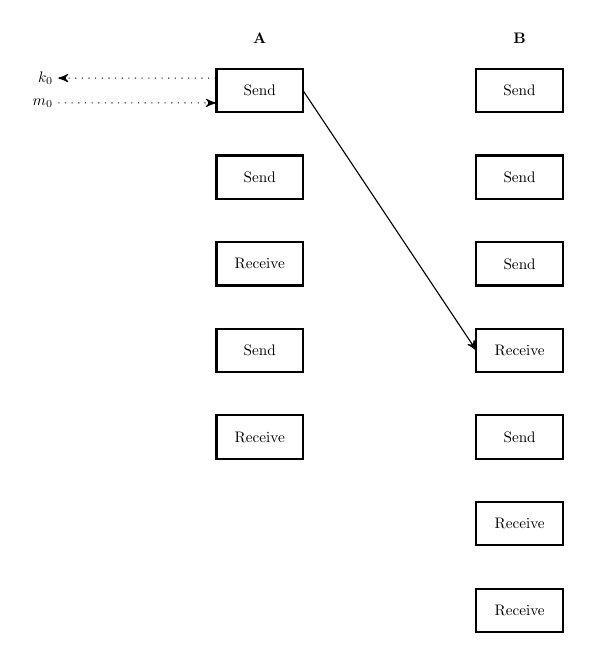
\begin{tikzpicture}[
  box/.style={rectangle,draw,inner sep=5pt,minimum height=1cm,minimum width=2cm,thick},
  node distance=2cm,
  ->,>=stealth',
  scale=0.55, every node/.style={scale=0.55}
]

  % Box t0
  \node [box] (t0) {Send};
  \node [coordinate,right of=t0,node distance=1cm] (tl0) {};
  \node [coordinate,above left=-0.125cm and 0cm of t0,node distance=1cm] (ta0) {};
  \node [left=2cm of ta0] (taa0) {$k_0$};
  \path (ta0) edge[dotted] node [] {} (taa0);
  \node [coordinate,below left=-0.125cm and 0cm of t0,node distance=1cm] (tb0) {};
  \node [left=2cm of tb0] (tbb0) {$m_0$};
  \path (tbb0) edge[dotted] node [] {} (tb0);


  \node [box,below of=t0] (t1) {Send};
  \node [box,below of=t1] (t2) {Receive};
  \node [box,below of=t2] (t3) {Send};
  \node [box,below of=t3] (t4) {Receive};

  \node [box,right of=t0,node distance=6cm] (t5) {Send};
  \node [box,below of=t5] (t6) {Send};
  \node [box,below of=t6] (t7) {Send};
  \node [box,below of=t7] (t8) {Receive};
  \node [box,below of=t8] (t9) {Send};
  \node [box,below of=t9] (t10) {Receive};
  \node [box,below of=t10] (t11) {Receive};

  \node [coordinate,left of=t8,node distance=1cm] (tl8) {};
  \path (tl0) edge[] node [] {} (tl8);

  \node [above=0.25cm of t0] (alice) {\bfseries{A}};
  \node [above=0.25cm of t5] (bob) {\bfseries{B}};
\end{tikzpicture} 
  \end{figure}
\end{frame}

\subsection{Security}
\label{sec:security}

\begin{frame}{Security I.}
  \begin{itemize}
  \item Forward security.
    \begin{itemize}
    \item Protect past states from current state leakages.
    \end{itemize}
  \item Post-compromise security (future secrecy).
    \begin{itemize}
    \item Protect future state from current state leakages.
    \end{itemize}
  \item Assert security through key- or ciphertext-indistinguishability games.
  \end{itemize}
\end{frame}

\begin{frame}{Security II.}
  \begin{figure}[ht]
      \centering
      \setlength{\fboxsep}{10pt}
      \scalebox{0.7}{%
      \fbox{%
         \algrenewcommand\textproc{}
 \algrenewcommand\algorithmicprocedure{\textbf{Game}}

 \begin{minipage}{.5\linewidth}
   \begin{algorithmic}[1]
     \Procedure{$\t{KIND}_b^\mathcal{A}$}{}
     \State $(\t{st}_\t{A},\t{st}_\t{B}) \gets$ \Call{Init}{$1^\lambda$}
     \State $b' \gets \mathcal{A}^{\t{RATCH,EXP,TEST}}$
     \State \Return $b'$
     \EndProcedure
   \end{algorithmic}
 \end{minipage}

 \vline

 \algrenewcommand\textproc{}
 \algrenewcommand\algorithmicprocedure{\textbf{Oracle}}

 \begin{minipage}{.5\linewidth}
   \begin{algorithmic}[1]
     \Procedure{TEST}{$\t{P}$}
     \If{$b = 1$}
     \State \Return $k_\t{P}$
     \EndIf
     \State \Return random $\{0,1\}^{|k_\t{P}|}$ 
     \EndProcedure

     \item[] % Blank line.

     \Procedure{EXP}{$\t{P}$}
     \State \Return $\t{st}_\t{P}$ 
     \EndProcedure
  \end{algorithmic}
\end{minipage}%

      }
    }
  \end{figure}

  \begin{figure}[ht]
      \centering
      \setlength{\fboxsep}{10pt}
      \scalebox{0.7}{%
      \fbox{%
        \algrenewcommand\textproc{}
  \algrenewcommand\algorithmicprocedure{\textbf{Game}}

  \begin{minipage}{.5\linewidth}
    \begin{algorithmic}[1]
      \Procedure{$\t{CIND}_b^\mathcal{A}$}{}
      \State $(\t{st}_\t{A},\t{st}_\t{B}) \gets$ \Call{Init}{$1^\lambda$}
      \State $b' \gets \mathcal{A}^{\t{RATCH',EXP}}$
      \State \Return $b'$
      \EndProcedure
    \end{algorithmic}
  \end{minipage}

  \vline

  \algrenewcommand\textproc{}
  \algrenewcommand\algorithmicprocedure{\textbf{Oracle}}

  \begin{minipage}{.5\linewidth}
    \begin{algorithmic}[1]
      \Procedure{RATCH'}{$\t{P},m_0,m_1$}
      \State \Return \Call{RATCH}{$\t{P},m_b$}
      \EndProcedure

      \item[] % Blank line.

      \Procedure{EXP}{$\t{P}$}
      \State \Return $\t{st}_\t{P}$ 
      \EndProcedure
   \end{algorithmic}
 \end{minipage}%

      }
    }
  \end{figure}
\end{frame}

\begin{frame}{Security III.}
  \begin{itemize}
  \item Powerful adversary.
  \item Many many attacks that lead to trivial victories.
  \item Games have to be adapted to exclude these attacks.
  \item The fewer attacks a game disallows the securer the protocol.
  \item Assess advantage of any adversary.
\[
  \t{Adv}(\mathcal{A}) = \left| \Pr \left[ \t{\{C,K\}IND}_0^\mathcal{A} \rightarrow 1 \right] -
                                \Pr \left[ \t{\{C,K\}IND}_1^\mathcal{A} \rightarrow 1 \right]
                         \right|.
\]
  \end{itemize}
\end{frame}

\section{Protocols}
\label{sec:protocols}

\subsection{Timeline}
\label{sec:timeline}

\begin{frame}{Timeline I.}
  \begin{enumerate}
  \item \textbf{2012.} Off-the-record messaging protocol.
  \item \textbf{2014.} Signal protocol.
  \item \textbf{2017.} Security analysis of Signal.
  \item \textbf{2017.} Bellare {\em et al.} Formalization of ratcheting. First
    limited, unidirectional protocol.
  \end{enumerate}
\end{frame}

\begin{frame}{Timeline II.}
  \begin{enumerate}
  \item \textbf{05/2018.} Poettering and Rösler. Optimally secure bidirectional
    key-agreement protocol (BRKE).
  \item \textbf{06/2018.} Jager and Stepanovs. Optimally secure messaging protocol.
  \item \textbf{09/2018.} Durak and Vaudenay. Sub-optimally secure, efficient key-agreement
    protocol (BARK).
  \item \textbf{10/2018.} Jost, Maurer and Mularczyk. Almost-optimally secure messaging
    protocol.
  \item \textbf{10/2018.} Alwen, Coretti and Dodis. Modularization of Signal Double
    Ratchet.
  \end{enumerate}
\end{frame}


% \begin{frame}{Security}
% \begin{columns}
% \column{0.6\linewidth}
%   \begin{figure}[ht]
%     \centering
%     \setlength{\fboxsep}{10pt}
%     \scalebox{0.5}{%
%     \fbox{%
%       \algrenewcommand\textproc{}
\algrenewcommand\algorithmicprocedure{\textbf{func}}

\begin{minipage}{1.2\linewidth}
  {\fontsize{8}{10}\selectfont
    \begin{multicols}{2}
  \begin{algorithmic}[1]
    \Procedure{Receive}{$ST,ad,C$}
    \State $(R,S) \gets ST$
    \State $(PK,E_\t{S},s,L_\t{S},vfk,K_\t{S},t_\t{S}) \gets S$
    \State $t^* \gets ad||C, \ t_\t{S} \gets t_\t{S} t^*, \ C || \sigma \gets C$
    \State \textbf{assert} \Call{\texttt{DS.Verify}}{$vfk,ad||C,\sigma$}
    \State $r||pk^*||vfk||C \gets C$
    \State $L\t{S}[...,(r-1)] \gets \perp$
    \For{$s' \gets r+1$  to $s$}
    \State $pk^* \gets$ \Call{\texttt{ku-KEM.UpdPk}}{$pk^*,L\t{S}[s']$}
    \EndFor
    \State $E_\t{S}^\dashv \gets E_\t{S}^\dashv+1, \ PK[E_\t{S}^\dashv] \gets pk^*$
    \State $S \gets (PK,E_\t{S},s,L_\t{S},vfk,K_\t{S},t_\t{S})$
    \State $(SK,E_\t{R},r,L_\t{R},sgk,K_\t{R},t_\t{R}) \gets R$
    \State $k^* \gets \perp, \ e||C \gets C$
    \State $t_\t{R} \gets t_\t{R} || L_\t{R}[E_\t{R}^\vdash+1]||...||L_\t{R}[e]$
    \State $L_\t{R}[...,e] \gets \perp$
    \For{$e' \gets E_\t{R}^\vdash$ to $e$}
    \State $c||C \gets C$
    \State $k \gets$ \Call{\texttt{ku-KEM.Dec}}{$SK[e'],c$}
    \State $k^* \gets k^* ||k$
    \EndFor
    \State $t_\t{R} \gets t_\t{R}||t^*$
    \State $k.o || K_\t{S} || k.m || sk \gets$ \Call{\texttt{H}}{$K_\t{R},k^*,L_\t{R}$}
    \State $SK[...,(e -1)] \gets \perp, \ SK[e] \gets sk$
    \For{$e' \gets e+1$  to $E_\t{R}^\dashv$}
    \State $SK[e'] \gets$ \Call{\texttt{ku-KEM.UpdSk}}{$SK[e'],t^*$}
    \EndFor
    \State $E_\t{R}^\vdash \gets e, \ r \gets r+1$
    \State $R_\t{u} \gets (SK_\t{u},E,r,L_\t{R},sgk_\t{u},K_\t{u},t)$
    \State $ST \gets (R,S)$
    \State \Return $(ST,k.o)$ 
    \EndProcedure
  \end{algorithmic}
  \end{multicols}
  }
\end{minipage}
%     }
%   }
% \end{figure}

% \column{0.5\linewidth}
% \begin{itemize}
%   \item asdfsa
%   \item saldfjasf
%   \item sdlfkjsadf l
% \end{itemize}

% \end{columns}
% \end{frame}

% \section{Protocols}
% \label{sec:protocols}

% \section{Benchmarks}
% \label{sec:benchmarks}

% \section{Conclusion}
% \label{sec:conclusion}

\end{document}
